\documentclass[runningheads]{llncs}
\pdfoutput=1
\usepackage[utf8]{inputenc}
\usepackage{amsmath}
\usepackage{amssymb}
\usepackage{mathpartir}
\usepackage{hyperref}
\usepackage{listings}
\usepackage{graphicx}
\lstdefinelanguage{michelson}{
  basicstyle=\fontsize{8}{9.6}\selectfont,
  morekeywords={parameter,storage,or,unit,mutez,pair,bool,address}, sensitive=false,
  morecomment=[l]{\#},
  morecomment=[\STACK]{/*}{*/},
  morestring=[b]",
}
\lstset{
  language=Caml,
  captionpos=b,
  aboveskip=-\smallskipamount,
  belowskip=-\smallskipamount,
  belowcaptionskip=0pt,
  basicstyle=\fontsize{8}{9.6}\selectfont,
  morekeywords={val}
}

%% structure
\newcommand{\Angle}[1]{\langle#1\rangle}

%% values
\newcommand{\NEG}{\neg}
\newcommand{\CNF}{\wedge}
\newcommand{\DNF}{\vee}
\newcommand{\TRUE}{\text{True}}
\newcommand{\FALSE}{\text{False}}
\newcommand{\EMPTYSTRING}{\text{$""$}}
\newcommand{\STACKCONCAT}{\text{$::$}}
\newcommand{\ZERO}{\text{0}}
\newcommand{\ONE}{\text{1}}
\newcommand{\VAMOUNT}{\text{amount}}
\newcommand{\VCONTRACT}{\text{contract}}

%% contract constants
\newcommand{\CAMOUNT}{\text{amount}}
\newcommand{\CBALANCE}{\text{balance}}
\newcommand{\CSENDER}{\text{sender}}
\newcommand{\CSOURCE}{\text{source}}
\newcommand{\CNOW}{\text{now}}
\newcommand{\CLEVEL}{\text{level}}
\newcommand{\CCHAINID}{\text{chain-id}}
\newcommand{\CSELF}{\text{self}}
\newcommand{\CSELFADDRESS}{\text{self-address}}
\newcommand{\CTOTALVOTINGPOWER}{\text{total-voting-power}}
\newcommand{\CVOTINGPOWER}{\text{voting-power}}

%% contract instructions
\newcommand{\AMOUNT}{\text{AMOUNT}}
\newcommand{\BALANCE}{\text{BALANCE}}
\newcommand{\SENDER}{\text{SENDER}}
\newcommand{\SOURCE}{\text{SOURCE}}
\newcommand{\NOW}{\text{NOW}}
\newcommand{\LEVEL}{\text{LEVEL}}
\newcommand{\CHAINID}{\text{CHAIN-ID}}
\newcommand{\SELF}{\text{SELF}}
\newcommand{\SELFADDRESS}{\text{SELF-ADDRESS}}
\newcommand{\TOTALVOTINGPOWER}{\text{TOTAL-VOTING-POWER}}
\newcommand{\VOTINGPOWER}{\text{VOTING-POWER}}
\newcommand{\MinusBalanceAmount}{\text{BALANCE-AMOUNT}}
%% auction contract
\newcommand{\AuctionOwner}{\text{auction-owner}}
\newcommand{\AuctionBidder}{\text{auction-bidder}}
\newcommand{\AuctionClose}{\text{auction-close}}
\newcommand{\AuctionOpen}{\text{auction-open}}
\newcommand{\AuctionBid}{\text{auction-bid}}

%% system definition
\newcommand{\VAL}{\textbf{v}}
\newcommand{\VAR}{\textbf{x}}
\newcommand{\VARIABLE}{\text{$Var$}}
\newcommand{\CONSTANT}{\text{$Const$}}
\newcommand{\TERM}{\text{$T$}}
\newcommand{\VariableX}{\text{$x$}}
\newcommand{\VariableV}{\text{$v$}}
\newcommand{\VariableK}{\text{$k$}}
\newcommand{\VariableA}{\text{$a$}}
\newcommand{\VariableB}{\text{$b$}}
\newcommand{\ELT}{\text{$Elt$}}
\newcommand{\A}{\text{$A$}}
\newcommand{\B}{\text{$B$}}
\newcommand{\N}{\text{$n$}}
\newcommand{\K}{\text{$k$}}
\newcommand{\V}{\text{$v$}}
\newcommand{\M}{\text{$m$}}
\newcommand{\VariableOne}{\text{$x_1$}}
\newcommand{\VariableTwo}{\text{$x_2$}}
\newcommand{\VariableN}{\text{$x_n$}}
\newcommand{\Constant}{\text{$c$}}
\newcommand{\ConstantOne}{\text{$c_1$}}
\newcommand{\ConstantTwo}{\text{$c_2$}}
\newcommand{\ConstantN}{\text{$c_n$}}
\newcommand{\LIST}{\text{$l$}}
\newcommand{\EMPTYLIST}{\text{$\{\}$}}
\newcommand{\TLIST}{\text{$l'$}}
\newcommand{\HEAD}{\text{$hd$}}
\newcommand{\TAIL}{\text{$tl$}}
\newcommand{\STAIL}{\text{$< tl >$}}
\newcommand{\Term}{\text{$t$}}
\newcommand{\TermOne}{\text{$t_1$}}
\newcommand{\TermTwo}{\text{$t_2$}}
\newcommand{\TermN}{\text{$t_n$}}
\newcommand{\TermB}{\text{$t_b$}}
\newcommand{\STACK}{\text{$S$}}
\newcommand{\EMPTYSTACK}{\text{[ ]}}
\newcommand{\STACKONE}{\text{$S$}}
\newcommand{\STACKTWO}{\text{$S$}}
\newcommand{\STACKN}{\text{$S$}}
\newcommand{\Stack}{\text{$s$}}
\newcommand{\StackOne}{\text{$s_1$}}
\newcommand{\StackTwo}{\text{$s_2$}}
\newcommand{\StackN}{\text{$s_n$}}
\newcommand{\TSTACK}{\text{$S'$}}
\newcommand{\TStack}{\text{$s'$}}
\newcommand{\STATE}{\text{$ST$}}
\newcommand{\STATEONE}{\text{$ST_1$}}
\newcommand{\STATETWO}{\text{$ST_2$}}
\newcommand{\STATEN}{\text{$ST_n$}}
\newcommand{\SYSTEM}{\text{$SE$}}
\newcommand{\INSTRUCTION}{\text{$I$}}
\newcommand{\TINSTRUCTION}{\text{$I'$}}
\newcommand{\INSTRUCTIONONE}{\text{$I1$}}
\newcommand{\INSTRUCTIONTWO}{\text{$I2$}}
\newcommand{\Instruction}{\text{$i$}}
\newcommand{\TInstruction}{\text{$i'$}}
\newcommand{\InstructionOne}{\text{$i_1$}}
\newcommand{\InstructionTwo}{\text{$i_2$}}
\newcommand{\InstructionN}{\text{$i_n$}}
\newcommand{\Invariant}{\text{$Iv$}}
\newcommand{\PREDICATE}{\text{$P$}}
\newcommand{\PREDICATEA}{\text{$P_A$}}
\newcommand{\PREDICATEB}{\text{$P_B$}}
\newcommand{\Predicate}{\text{$p$}}
\newcommand{\Failwith}{\text{$Failwith$}}
\newcommand{\PredicateOne}{\text{$p_1$}}
\newcommand{\PredicateTwo}{\text{$p_2$}}
\newcommand{\PredicateN}{\text{$p_n$}}
\newcommand{\SETA}{\text{$\mathcal{A}$}}
\newcommand{\SETAAUCTION}{\text{$\mathcal{A}_{auction}$}}
\newcommand{\SETPOST}{\text{$\mathcal{A'}$}}
\newcommand{\SETPOSTAUCTION}{\text{$\mathcal{A'}_{auction}$}}
\newcommand{\EMPTY}{\text{$\O$}}
\newcommand{\PCreate}{\text{$P_{Create}$}}
\newcommand{\PBidding}{\text{$P_{Bidding}$}}
\newcommand{\PClose}{\text{$P_{Close}$}}
\newcommand{\SE}{\text{SE}}
\newcommand{\SINIT}{\text{$s_{init}$}}
\newcommand{\SFINAL}{\text{$s_{final}$}}
\newcommand{\FMAP}{\textbf{map}}
\newcommand{\MAPA}{\textbf{$map_A$}}
\newcommand{\MAPB}{\textbf{$map_B$}}
\newcommand{\MapBidding}{\textbf{$map_{bidding}$}}
\newcommand{\MapCreate}{\textbf{$map_{create}$}}
\newcommand{\MapClose}{\textbf{$map_{close}$}}
\newcommand{\MAPER}{\text{$\overline{\textbf{map}}$}}


%% operation
\newcommand{\CONS}{\text{cons}}
\newcommand{\NIL}{\text{nil}}
\newcommand{\PLUS}{\textbf{+}}
\newcommand{\MINUS}{\textbf{-}}
\newcommand{\EQUAL}{\textbf{=}}
\newcommand{\LESS}{\textbf{$<$}}
\newcommand{\LESSEQUAL}{\textbf{$<=$}}
\newcommand{\MORE}{\textbf{$>$}}
\newcommand{\MOREEQUAL}{\textbf{$>=$}}

%% instructions
\newcommand{\UNIT}{\text{Unit}}
\newcommand{\PAIR}{\text{Pair}}
\newcommand{\LEFT}{\text{Left}}
\newcommand{\RIGHT}{\text{Right}}
\newcommand{\SOME}{\text{Some}}
\newcommand{\NONE}{\text{None}}
\newcommand{\ADD}{\text{ADD}}
\newcommand{\DROP}{\text{DROP}}
\newcommand{\LOOP}{\text{LOOP}}
\newcommand{\FAILWITH}{\text{FAILWITH}}
\newcommand{\TRANSFER}[2]{\text{Transfer($#1$, $#2$)}}
\newcommand{\CONTRACT}{\text{CONTRACT}}
\newcommand{\CAR}{\text{CAR}}
\newcommand{\EXEC}{\text{EXEC}}
\newcommand{\APPLY}{\text{APPLY}}
\newcommand{\IF}{\text{IF}}
\newcommand{\IFLEFT}{\text{IF-LEFT}}
\newcommand{\IFRIGHT}{\text{IF-RIGHT}}
\newcommand{\IFCONS}{\text{IF-CONS}}
\newcommand{\ITER}{\text{ITER}}
\newcommand{\TITER}{\text{ITER'}}
\newcommand{\DIG}{\text{DIG}}
\newcommand{\DIP}{\text{DIP}}
\newcommand{\DIPN}{\text{DIP n}}
\newcommand{\TDIP}{\text{DIP'}}
\newcommand{\ABS}{\text{ABS}}
\newcommand{\COMPARE}{\text{COMPARE}}
\newcommand{\TCOMPARE}{\text{COMPARE'}}
\newcommand{\HASHKEY}{\text{HASH-KEY}}
\newcommand{\CONCAT}{\text{CONCAT}}
\newcommand{\TCONCAT}{\text{CONCAT'}}
\newcommand{\MEN}{\text{MEN}}
\newcommand{\TMEN}{\text{MEN'}}
\newcommand{\TMAP}{\text{MAP'}}
\newcommand{\PUSH}{\text{PUSH}}
\newcommand{\XOR}{\text{XOR}}
\newcommand{\MAP}{\textbf{MAP}}
\newcommand{\LAMBDA}{\text{LAMBDA}}


%symbols
\newcommand{\Overline}[1]{\text{$\overline{#1}$}}
\newcommand{\Mapsto}{\text{$\mapsto$}}
\newcommand{\Mid}{\text{$\mid$}}
\newcommand{\Mathcal}[1]{\text{$\mathcal{#1}$}}
\newcommand{\Models}{\text{$\models$}}
\newcommand{\SRightarrow}{\text{$\rightarrow$}}
\newcommand{\NSRightarrow}{\text{$\nrightarrow$}}
\newcommand{\Wedge}{\text{$\wedge$}}
\newcommand{\At}{\text{$@$}}
\newcommand{\Subseteq}{\text{$\subseteq$}}
\newcommand{\Vee}{\text{$\vee$}}
%\newcommand{\Cup}{\text{$\cup$}}
\newcommand{\STRINGCONCAT}{\text{$\hat{}$}}
\newcommand{\DOT}{\text{$...$}}


%% functions
\newcommand{\FABS}[1]{\text{abs($#1$)}}
\newcommand{\FXOR}{\text{xor}}
\newcommand{\FHASHKEY}[1]{\text{hash-key($#1$)}}
\newcommand{\FCONCAT}[1]{\text{concat($#1$)}}
\newcommand{\FGetTy}[1]{\text{get-ty($#1$)}}
\newcommand{\FLEN}[1]{\text{len($#1$)}}
\newcommand{\FAND}{\text{and}}
\newcommand{\FOR}{\text{or}}
\newcommand{\FNOT}{\text{not}}
\newcommand{\GETCONTRACTTYPE}{\text{get-contract-type}}
\newcommand{\UNOP}{\text{unop}}
\newcommand{\BINOP}{\text{binop}}



%% transition relations
\newcommand{\StateTrans}{\text{$\longrightarrow_S$}}
\newcommand{\ExprTrans}{\text{$\longrightarrow_E$}}
\newcommand{\SystemTrans}{\text{$\longrightarrow$}}


%% types
\newcommand\TEnv{\Gamma}
\newcommand\JTypeCode[2]{\vdash_C#1 : #2}
\newcommand\JTypeValue[2]{\vdash_V#1 : #2}
\newcommand\JTypeExpr[3]{#1 \vdash #2 : #3}
\newcommand{\TY}{\text{ty}}
\newcommand{\TYF}{\text{ty$_{1}$}}
\newcommand{\TYS}{\text{ty$_{2}$}}
\newcommand{\TYT}{\text{ty$_{3}$}}
\newcommand{\TYA}{\text{A}}
\newcommand{\TYB}{\text{B}}
\newcommand{\TYC}{\text{C}}
%% standard types
\newcommand{\TBOOL}{\text{bool}}
\newcommand{\TOR}{\text{or}}
\newcommand{\TYLIST}{\text{list}}
\newcommand{\TUNIT}{\text{unit}}
\newcommand{\TPAIR}{\text{pair}}
\newcommand{\TOPTION}{\text{option}}
\newcommand{\TMUTEZ}{\text{mutez}}
\newcommand{\TSTR}{\text{string}}
\newcommand{\TINT}{\text{int}}
\newcommand{\TNAT}{\text{nat}}
\newcommand{\TKEY}{\text{key}}
\newcommand{\TKEYHASH}{\text{key-hash}}
\newcommand{\TSIG}{\text{signature}}
\newcommand{\TADDR}{\text{address}}
\newcommand{\TTIME}{\text{timestamp}}
\newcommand{\TCONTRACT}{\text{contract}}
\newcommand{\TCHAINID}{\text{chain-id}}
\newcommand{\TLAMBDA}{\text{lambda}}







%% typing related
\newcommand{\EmptyEnv}{\cdot}

%% evaluation contexts
\newcommand\EC[1]{\epsilon[#1]}

%% metavariables


%%% Local Variables:
%%% mode: latex
%%% TeX-master: "paper"
%%% End:



\begin{document}
%
\title{Symblic Execusion Model}
%
%\titlerunning{Abbreviated paper title}
% If the paper title is too long for the running head, you can set
% an abbreviated paper title here
%
\author{Thi Thu Ha Doan\orcidID{0000-0001-7524-4497}\and
  Peter Thiemann\orcidID{0000-0002-9000-1239}}

%
\authorrunning{Ha Doan, P. Thiemann}
% First names are abbreviated in the running head.
% If there are more than two authors, 'et al.' is used.
%
\institute{University of Freiburg, Germany \\
  \email{\{doanha,thiemann\}@informatik.uni-freiburg.de}
}
%
\maketitle              % typeset the header of the contribution
%
\begin{abstract}
 

\keywords{}
\end{abstract}

%
%
%
\section{Introduction}
\label{sec:introduction}
\section{Symblic Execution Model}
\label{sec:symblic-execution-model}
\subsection{Models}
%Let \VARIABLE\ = \{\VariableOne, \VariableTwo, \DOT\ \} is a set of variables.\\
%Let \CONSTANT\ = \{\BALANCE, \AMOUNT, \SENDER, \SOURCE, \NOW, \LEVEL, \CHAINID, \SELF, \ConstantOne, \ConstantTwo, \DOT\ \} is a set of constants.\\
%Let \Term\ is a term that ranges over variables and constants.\\
Let \STACK\ = \TermOne\ \STACKCONCAT\ \TermTwo\ \STACKCONCAT\ \DOT\ \STACKCONCAT\ \EMPTYSTACK\ is a stack, where elements are terms.
\\
Let \INSTRUCTION\ = \InstructionOne; \InstructionTwo; \DOT; \InstructionN\ is a sequence of intructions. 
\\
Let \PREDICATE\ is a predicate. 

\begin{definition}
A system state of the symbolic execusion is described as a tuple \STATE\ = [\INSTRUCTION, \STACK, \TSTACK, \PREDICATE], where \STACK\ is the main stack and \TSTACK\ is a temporary stack.
\end{definition}

Let \SYSTEM\ = \{\STATEONE, \STATETWO, \DOT, \STATEN \} be the set of system states.
\\
\\
Let $S_{init}$  be the initial state. 

\begin{itemize}
\item[]  $S_{init}$ = (Pair $Pa$ \Term) \STACKCONCAT\ \EMPTYSTACK
\end{itemize}


\noindent Let $S_{final}$  be the final state. 

\begin{itemize}
\item[]  $S_{final}$ = (\PAIR\ $ops$ $t'$) \STACKCONCAT\ \EMPTYSTACK
\end{itemize}

%Where $t$ and $t'$ represent the storage and have the same structure.

%Postcondition

%(t.x = t'.x)

\pagebreak

\begin{figure}
\begin{align*}
T, U &::= \\
   &\Mid\ < \text{comparable type}> \\
   &\Mid\ \text{option} <\text{type}> \\
   &\Mid\ \text{list} <\text{type}> \\
   &\Mid\ \text{set} <\text{comparable type}> \\
   &\Mid\ \text{operation} \\
   &\Mid\ \text{contract} <\text{type}> \\
   &\Mid\ \text{ticket} <\text{comparable type}> \\
   &\Mid\ \text{pair} <\text{type}> <\text{type}> \\
   &\Mid\ \text{or} <\text{type}> <\text{type}> \\
   &\Mid\ \text{lambda} <\text{type}> <\text{type}> \\
   &\Mid\ \text{map} <\text{comparable type}> <\text{type}> \\
   &\Mid\ \text{big-map} <\text{comparable type}> <\text{type}> \\
   &\Mid\ \text{bls12-381-g1} \\
   &\Mid\ \text{bls12-381-g2} \\
   &\Mid\ \text{bls12-381-fr} \\
   &\Mid\ \text{sapling-transaction} <\text{natural number constant}> \\
   &\Mid\ \text{sapling-state} <\text{natural number constant}> \\
   &\Mid\ \text{chest} \\
   &\Mid\ \text{chest-key} \\
<\text{comparable type}> ::= \\
   &\Mid\ \text{unit} \\
   &\Mid\ \text{never} \\
   &\Mid\ \text{bool} \\
   &\Mid\ \text{int}\\
   &\Mid\ \text{nat}\\
   &\Mid\ \text{string}\\
   &\Mid\ \text{chain-id}\\
   &\Mid\ \text{bytes}\\
   &\Mid\ \text{mutez}\\
   &\Mid\ \text{key-hash}\\
   &\Mid\ \text{key}\\
   &\Mid\ \text{signature}\\
   &\Mid\ \text{timestamp}\\
   &\Mid\ \text{address}\\
   &\Mid\ \text{tx-rollup-l2-address}\\
   &\Mid\ \text{option} <\text{comparable type}>\\
   &\Mid\ \text{or} <\text{comparable type}> <\text{comparable type}>\\
   &\Mid\ \text{pair} <\text{comparable type}> <\text{comparable type}> \DOT \\
\end{align*}
\caption{Types}
\label{fig:type}
\end{figure}

\pagebreak
\begin{figure}
\begin{align*}
\text{t} &::= \\
   &\Mid\ < \text{variable} > \\
   &\Mid\ < \text{account constant} > \\
   &\Mid\ < \text{int constant} > \\
   &\Mid\ < \text{string constant} > \\
   &\Mid\ < \text{byte sequence constant} > \\
   &\Mid\ \UNIT \\
   &\Mid\ \TRUE \\
   &\Mid\ \FALSE \\
   &\Mid\ \PAIR\ \text{t1 t2}\\
   &\Mid\ \LEFT\ \text{t}\\
   &\Mid\ \RIGHT\ \text{t}\\ 
   &\Mid\ \SOME\ \text{t}\\
   &\Mid\ \NONE \\
   &\Mid\ \text{\{t ; ... \}}\\
   &\Mid\ \text{\{ Elt t1 t2 ; ... \}}\\
   &\Mid\ <\text{instruction}>   \\
< \text{variable} > &::= \\ 
   &\Mid\ \VAR\\
< \text{account constant} > &::= \\ 
   &\Mid\ \text{balance} \\
   &\Mid\ \text{amount} \\
   &\Mid\ \text{sender} \\
   &\Mid\ \text{source} \\
   &\Mid\ \text{now} \\
   &\Mid\ \text{level} \\
   &\Mid\ \text{chain-id} \\
   &\Mid\ \text{self}  \\
   &\Mid\ \text{self-address}  \\
   &\Mid\ \text{total-voting-power}  \\
   &\Mid\ \text{voting-power}  \\
< \text{natural number constant} > &::= \\ 
   &\Mid\ \text {[0-9]+} \\
< \text{int constant} > &::= \\
  &\Mid\ < \text{natural number constant} > \\
  &\Mid\ \text{-} < \text{natural number constant} > \\
<\text{string constant}> &::= \\
  &\Mid\ \text{"} < \text{string content}>\text{*"} \\
<\text{instruction}> &::= \\
  &\Mid\ \DROP \\
  &\Mid\ \DROP <\text{natural number constant}> \\
  &\text{...}
\end{align*}
\caption{Terms}
\label{fig:term}
\end{figure}


\pagebreak
\begin{figure}
\begin{align*}
\text{p} &::= \\
   &\Mid\ < \text{atomic formula} > \\
   &\Mid\ \NEG\ \text{p} \
   \Mid\ \text{p}\ \CNF\ \text{q} \
   \Mid\ \text{p}\ \DNF\ \text{q} \\
< \text{atomic formula} > &::= \\ 
    &\Mid\ < \text{buop} > < \text{bterm} >\\ 
   &\Mid\  < \text{bterm} >  < \text{biop} > < \text{bterm} >\\ 
< \text{butop} > &::= \\
   &\Mid\ \text{not} \\
< \text{biop} > &::= \\
   &\Mid\ \text{$=$} \
   \Mid\ \text{$>$} \
   \Mid\ \text{$<$} \
   \Mid\ \text{$>=$} \
   \Mid\ \text{$=<$} \
   \Mid\ \text{$!=$} \\
   &\Mid\ \text{and}\ \Mid\ \text{or}\ \Mid\ \text{xor}\\
< \text{bterm} > &::= \\ 
   &\Mid\ \text{t} \\
   &\Mid\ < \text{unop} > \text{t} \\ 
   &\Mid\ \text{t}\ < \text{binop} > \text{t}\\  
< \text{utop} > &::= \\ 
   &\Mid\ \text{abs} \\
   &\Mid\ \text{size} \\
   &\Mid\ \text{int} \\
   &\Mid\ \text{contract}  < \text{type} > \\
   &\Mid\ \text{isleft} \\
   &\Mid\ \text{isnone} \\
   &\Mid\ \text{neg} \\
   &\Mid\ \text{blake2b} \\
   &\Mid\ \text{hash-key} \\
   &\Mid\ \text{keccak} \\
   &\Mid\ \text{pairing-check} \\
   &\Mid\ \text{sha256} \\
   &\Mid\ \text{sha3} \\
   &\Mid\ \text{sha512} \\
   &\Mid\ \text{implicit-account} \\
   &\Mid\ \text{check-sig} \\
< \text{bitop} > &::= \\ 
   &\Mid\ \text{+}\ \Mid\ \text{-}\ \Mid\ \text{*}\ \Mid\ \text{/}
\end{align*}
\caption{Predicates}
\label{fig:predicate}
\end{figure}



%Let \SETA\ \Subseteq\ \VARIABLE\ \CUP\ \CONSTANT\ is a set of variables and constants that represents a initial stack. Namely, the initial state of main stack contains of only one element that is a term over \SETA.

%\SETA\ = \{\VariableOne, \VariableTwo, \DOT, \VariableN, \BALANCE, \AMOUNT, \SENDER, \SOURCE, \NOW, \LEVEL, \CHAINID, \SELF\}

%Example:Let us consider the auction contract.

%\SETAAUCTION\ = \{\AuctionBid, \AuctionOwner, \AuctionOpen, \AuctionBidder, \BALANCE, \AMOUNT, \SENDER, \SOURCE, \NOW, \LEVEL, \CHAINID, \SELF\}.

%\SINIT\ = \PAIR\ (\AuctionBidder\ (\PAIR\ \AuctionOpen\ (\PAIR\ \AuctionOwner\ \AuctionBidder))) \STACKCONCAT\ \EMPTYSTACK.

%\begin{definition}
%The function maps assign values to variables. 

%\FMAP : \SETA\  \Mapsto\ \TERM, where \MAP(\VariableX) = \Term\ is donated as (\VariableX\ \Mapsto\ \Term)
%\end{definition}

%To apply the map funtions to a set of variable, we introduce \MAPER.

%\begin{align*}
%\MAPER(\SETAAUCTION) = \{\VariableOne\ \Mapsto\ \TermOne, \VariableTwo\ \Mapsto\ \TermTwo, \DOT, \VariableN\ \Mapsto\ \TermN, \BALANCE\ \Mapsto\ \TermB \}. 
%\end{align*}

%When the execution is terminated, \PREDICATE\ is called the precondition of the execution and the postcondition is the appication of the map function to the initial stack.
%\begin{align*}
%\SETPOST\ = \Overline\MAP(\SETA)
%\end{align*}

%\paragraph{Example}
%\begin{align*}
%\SFINAL\ = \PAIR\ (\TRANSFER\MinusBalanceAmount\AuctionBidder)\\ (\PAIR\ \TRUE\ (\PAIR\ \AuctionOwner\ \SENDER))
%\end{align*}
%\begin{align*}
%\SETPOSTAUCTION\ = \Overline\MapBidding(\SETAAUCTION) = \\ \{\AuctionOwner\  \Mapsto\ \SETAAUCTION.\AuctionOwner,  \\ \AuctionOpen\ \Mapsto\ \TRUE, \\ \AuctionBidder\ \Mapsto\ \SETAAUCTION.\SENDER, \\ \BALANCE\ \Mapsto \SETAAUCTION.\AMOUNT\}
%\end{align*}

%\paragraph{Invariants.}
%\begin{definition}
%A predicate \Invariant\ is an invariant  iff (\SETA, \SETPOST, \PREDICATE) is a model of \Invariant.
%\begin{align*}
%(\SETA, \SETPOST,\PREDICATE)\ \Models\ \Invariant
%\end{align*}
%\end{definition}

%In another word, \PREDICATE[\SETA, \SETPOST]\Invariant.

%\paragraph{Example.}
%\begin{itemize}
%\item[] I1-constant-owner: (\SETPOSTAUCTION.\AuctionOwner\ \EQUAL\ \SETAAUCTION.\AuctionOwner)
%\item[] I2-higher-bidding: (\SETPOSTAUCTION.\AuctionBidder\ \EQUAL\  \SETAAUCTION.\SENDER)
%\end{itemize}
\pagebreak
\paragraph{Sequence actions.}
%\begin{definition}
%There is a step from an entrypoint \A\ to \B: \A\ \SRightarrow\ \B\  iff  there is a model for the application of the map \Overline\MAPA\ to the predicate \PREDICATEB: \Models\ \Overline\MAPA(\PREDICATEB).
%\end{definition}

%Example.

\begin{figure}[h]
\center
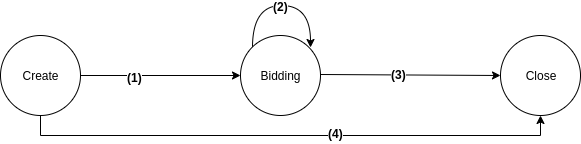
\includegraphics[width= 10 cm]{life-cycle-1}
\caption{Life-cycle for the auction contract.}
\label{fca1}
\end{figure} 

%\paragraph{Preconditions}
%\begin{itemize}
%\item[] \PCreate\ = \{\EMPTY\} 
%\item[] \PBidding\ = \{\AuctionOpen\ \EQUAL\ \TRUE, \AMOUNT\ \MORE\ \BALANCE\ \MINUS\ \AMOUNT\} 
%\item[] \PClose\ = \{\AuctionOpen\ \EQUAL\ \TRUE\}
%\end{itemize}


%\paragraph{Maps}
%\begin{itemize}
%\item[] \Overline\MapCreate\ = \{\AuctionOpen\ \Mapsto\ \TRUE,  \AuctionBidder\ \Mapsto\ \SENDER, \BALANCE\ \Mapsto\ \ZERO\}
%\item[] \Overline\MapBidding\ = \{\AuctionOwner \Mapsto\ \AuctionOwner, \AuctionOpen\ \Mapsto\ \TRUE,  \AuctionBidder\ \Mapsto\ \SENDER, \BALANCE\ \Mapsto\  \AMOUNT\}
%\item[] \Overline\MapClose\ = \{\AuctionOpen\ \Mapsto\ \FALSE, \BALANCE\ \Mapsto\ \ZERO\}
%\end{itemize}

%\begin{itemize}
%\item[(1)] ($\textbf{Create}$ \SRightarrow\ $\textbf{Bidding}$):
%\\ \Models\  \Overline\MapCreate(\PBidding) = \{\TRUE\ \EQUAL\ \TRUE, \AMOUNT\ \MORE\ \BALANCE\ - \AMOUNT\}
%\item[(2)] ($\textbf{Bidding}$ \SRightarrow\ $\textbf{Bidding}$) : 
%\\ \Models\  \Overline\MapBidding(\PBidding) = \{\TRUE\ \EQUAL\ \TRUE, \AMOUNT\ \MORE\ \AMOUNT'\ - \AMOUNT\}
%\item[(3)] ($\textbf{Bidding}$ \SRightarrow\ $\textbf{Close}$) : 
%\\ \Models\ \Overline\MapBidding(\PClose) = \{\TRUE\ \EQUAL\ \TRUE\}
%\item[(4)] ($\textbf{Create}$ \SRightarrow\ $\textbf{Close}$) : 
%\\ \Models\ \Overline\MapCreate(\PClose) \EQUAL\ \{\TRUE\ \EQUAL\ \TRUE\}
%\item[(5)] ($\textbf{Close}$ \NSRightarrow\ $\textbf{Bidding}$) : 
%\\ \Models\ \Overline\MapBidding(\PClose) = \{\FALSE\ \EQUAL\ \TRUE\}
%\end{itemize}
\pagebreak
\begin{figure}[tp]
\begin{mathpar}
  \inferrule{}{
      \JTypeExpr\TEnv{\VAR}{\TY} \\ \JTypeExpr\TEnv{\UNIT}{\TUNIT} \\ \JTypeExpr\TEnv{\TRUE}{\TBOOL} \\
\JTypeExpr\TEnv{\FALSE}{\TBOOL}
    }
\end{mathpar}

\begin{mathpar}
  \inferrule{}{
      \JTypeExpr\TEnv{\CBALANCE}{\TMUTEZ} \\ \JTypeExpr\TEnv{\CAMOUNT}{\TMUTEZ} \\ \JTypeExpr\TEnv{\CSENDER}{\TADDR} 
    }
\end{mathpar}

\begin{mathpar}
  \inferrule{}{
\JTypeExpr\TEnv{\CSOURCE}{\TADDR} \\
\JTypeExpr\TEnv{\CNOW}{\TTIME} \\
\JTypeExpr\TEnv{\CLEVEL}{\TNAT} \\
    }
\end{mathpar}

\begin{mathpar}
  \inferrule{}{
\JTypeExpr\TEnv{\CCHAINID}{\TCHAINID} \\
\JTypeExpr\TEnv{\CSELF}{\TCONTRACT\ \TY}
%\JTypeExpr\TEnv{\CSELFADDR}{\TADDR} \\
    }
\end{mathpar}

\begin{mathpar}
  \inferrule{\JTypeExpr\TEnv{\TermOne}{\TYF} \\ \JTypeExpr\TEnv{\TermTwo}{\TYS}}{
      \JTypeExpr\TEnv{\PAIR\ \TermOne\ \TermTwo}{\TPAIR\ \TYF\ \TYS}
    }
\end{mathpar}

\begin{mathpar}
  \inferrule{\JTypeExpr\TEnv{\TermOne}{\TYF}}{
      \JTypeExpr\TEnv{\LEFT\ \TermOne}{\TOR\ \TYF\ \TY}
    } 
    
    \inferrule{\JTypeExpr\TEnv{\TermOne}{\TYF}}{
      \JTypeExpr\TEnv{\RIGHT\ \TermOne}{\TOR\ \TY\ \TYF}
    }
    
     \inferrule{\JTypeExpr\TEnv{\TermOne}{\TYF}}{
      \JTypeExpr\TEnv{\SOME\ \TermOne}{\TOPTION\ \TYF}
    }
    
\end{mathpar}
  \caption{Typing rules for Terms}
  \label{fig:typing-rule}
\end{figure}

\pagebreak
\begin{figure}[tp]
\begin{mathpar}
  \inferrule{}{
      \JTypeExpr\TEnv{\EXE}{\TYF\ \STACKCONCAT\ \LAMBDA\ \TYF\ \TYS\ \STACKCONCAT\ \TYA\ \SRightarrow\ \TYS\ \STACKCONCAT\ \TYA}
    }
\end{mathpar}

\begin{mathpar}
  \inferrule{}{
      \JTypeExpr\TEnv{\APPLY}{\TYF\ \STACKCONCAT\ \LAMBDA\ (\PAIR\ \TYF\ \TYS)\ \TYT\ \STACKCONCAT\ \TYA\ \SRightarrow\ \LAMBDA\ \TYF\ \TYS\ \STACKCONCAT\ \TYA}
    }
\end{mathpar}

\begin{mathpar}
  \inferrule{\JTypeExpr\TEnv{\INSTRUCTIONONE}{\TYA\ \SRightarrow\ \TYB} \\ \JTypeExpr\TEnv{\INSTRUCTIONTWO}{\TYA\ \SRightarrow\ \TYB}
  }{
      \JTypeExpr\TEnv{\IF\ \INSTRUCTIONONE\ \INSTRUCTIONTWO}{\TBOOL\ \STACKCONCAT\ \TYA\ \SRightarrow\ \TYB}
    }
\end{mathpar}

\begin{mathpar}
  \inferrule{\JTypeExpr\TEnv{\INSTRUCTIONONE}{\TYA\ \SRightarrow\ \TYB} \\ \JTypeExpr\TEnv{\INSTRUCTIONTWO}{\TYA\ \SRightarrow\ \TYB}
  }{
      \JTypeExpr\TEnv{\IFLEFT\ \INSTRUCTIONONE\ \INSTRUCTIONTWO}{\TOR\ \TYF\ \TYS\ \STACKCONCAT\ \TYA\ \SRightarrow\ \TYB}
    }
\end{mathpar}

\begin{mathpar}
  \inferrule{\JTypeExpr\TEnv{\INSTRUCTIONONE}{\TYA\ \SRightarrow\ \TYB} \\ \JTypeExpr\TEnv{\INSTRUCTIONTWO}{\TYB\ \SRightarrow\ \TYC}
  }{
      \JTypeExpr\TEnv{\INSTRUCTIONONE\ ; \INSTRUCTIONTWO}{\TYA\ \SRightarrow\ \TYC}
    }
\end{mathpar}

\begin{mathpar}
  \inferrule{\JTypeExpr\TEnv{\INSTRUCTION}{\TY\ \STACKCONCAT\ \TYA\ \SRightarrow\ \TYA}
  }{
      \JTypeExpr\TEnv{\ITER\ \INSTRUCTION}{\TYLIST\ \TY\ \STACKCONCAT\ \TYA\ \SRightarrow\ \TYA}
    }
\end{mathpar}

\begin{mathpar}
  \inferrule{\JTypeExpr\TEnv{\INSTRUCTION}{\TYA\ \SRightarrow\ \TBOOL\ \STACKCONCAT\ \TYA}
  }{
      \JTypeExpr\TEnv{\LOOP\ \INSTRUCTION}{\TBOOL\ \STACKCONCAT\ \TYA\ \SRightarrow\ \TYA}
    }
\end{mathpar}

\begin{mathpar}
  \inferrule{\JTypeExpr\TEnv{\INSTRUCTION}{\TYA\ \SRightarrow\ \TYB}
  }{
      \JTypeExpr\TEnv{\DIP\ \INSTRUCTION}{\TY\ \STACKCONCAT\ \TYA\ \SRightarrow\ \TY\ \STACKCONCAT\ \TYB}
    }
\end{mathpar}

\begin{mathpar}
  \inferrule{\JTypeExpr\TEnv{\INSTRUCTION}{\TYA\ \SRightarrow\ \TBOOL\ \STACKCONCAT\ \TYA}
  }{
      \JTypeExpr\TEnv{\DIP\ \INSTRUCTION}{\TBOOL\ \STACKCONCAT\ \TYA\ \SRightarrow\ \TYA}
    }
\end{mathpar}

\begin{mathpar}
  \inferrule{}{
      \JTypeExpr\TEnv{\ADD}{\TNAT\ \STACKCONCAT\ \TNAT\ \STACKCONCAT\ \TYA\ \SRightarrow\ \TNAT\ \STACKCONCAT\ \TYA}
    }
\end{mathpar}

\begin{mathpar}
  \inferrule{
   \FLEN\A\ \EQUAL\ \N \\
  \JTypeExpr\TEnv{\INSTRUCTION}{\TYB\ \SRightarrow\ \TYC}
  }{
      \JTypeExpr\TEnv{\DIP\ \N\ \INSTRUCTION}{\TYA\ \At\ \TYB\ \SRightarrow\ \TYA\ \At\ \TYC}
    }
\end{mathpar}

  \caption{Typing rules for Rules}
  \label{fig:typing-rule}
\end{figure}

\pagebreak
\subsection{Rules}
The set of instructions is divided into two groups \INSTRUCTION\ and \TINSTRUCTION. Given an instruction \Instruction, \TInstruction\ is a copy version of \Instruction, where \Instruction\ operates on the main stack \STACK\ and \TInstruction\ operates only on the temporary stack \TSTACK.

The rule semantic is defined by several kinds of transitions:
\begin{enumerate}
\item \ExprTrans\ single-step evaluation of an expression in a system state,
\item \StateTrans\ internal transitions of a system state,
\item \SystemTrans\ synbolic system transitions.
\end{enumerate}



\subsubsection{System rules}
\begin{mathpar}
\inferrule[INVALID-PRE]
  { \NEG\ \PREDICATE
  }{
  \{[\INSTRUCTION, \STACK, \TSTACK, \PREDICATE], \SYSTEM]\} \SystemTrans\ \{\SYSTEM\}}
\end{mathpar}

\subsubsection{Instruction rules}
\paragraph{Control structures}
%EXE
\begin{mathpar}
  \inferrule[EXE]
  {  
  }{
    [(\EXE; \INSTRUCTION),  \StackOne\ \STACKCONCAT\ \{\INSTRUCTIONONE\} \STACKCONCAT\ \STACK, \TSTACK, \PREDICATE] \StateTrans\ [(\INSTRUCTIONONE; \INSTRUCTION), \StackOne\ \STACKCONCAT\ \STACK, \TSTACK, \PREDICATE]}
\end{mathpar}

%APPLY
\begin{mathpar}
  \inferrule[APPLY]
  {  
  }{
    \text{[(\APPLY; \INSTRUCTION), \StackOne\ \STACKCONCAT\ \{I1\} \STACKCONCAT\ \STACK, \TSTACK, \PREDICATE]} \StateTrans\ \text{[\INSTRUCTION, \{\PUSH\ \FGetTy\StackOne\ \StackOne; \PAIR; \INSTRUCTIONONE\} \STACKCONCAT\ \STACK, \TSTACK, \PREDICATE]}}
\end{mathpar}

%IF
\begin{mathpar}
  \inferrule[IF]
  {  
  }{
    \{[(\IF\ \INSTRUCTIONONE\  \INSTRUCTIONTWO; \INSTRUCTION),  \StackOne\ \STACKCONCAT\ \STACK, \TSTACK, \PREDICATE], \SYSTEM\} \SystemTrans\  \{[\INSTRUCTIONONE, \STACK, \TSTACK, \PREDICATE\ \Wedge\ \StackOne], [\INSTRUCTIONTWO, \STACK, \TSTACK, \PREDICATE\ \Wedge\ \NEG\ \StackOne], \SYSTEM\}}
\end{mathpar}


%IF-LEFT-LEFT
\begin{mathpar}
  \inferrule[IF-LEFT-LEFT]
  {  
  }{
    [(\IFLEFT\ \INSTRUCTIONONE\  \INSTRUCTIONTWO; \INSTRUCTION),  \LEFT\ \Term\ \STACKCONCAT\ \STACK, \TSTACK, \PREDICATE] \StateTrans\  [\INSTRUCTIONONE; \INSTRUCTION, \Term\ \STACKCONCAT\ \STACK, \TSTACK, \PREDICATE]}
\end{mathpar}

%IF-LEFT-RIGHT
\begin{mathpar}
  \inferrule[IF-LEFT-RIGHT]
  {  
  }{
    [(\IFLEFT\ \INSTRUCTIONONE\  \INSTRUCTIONTWO; \INSTRUCTION),  \RIGHT\ \Term\ \STACKCONCAT\ \STACK, \TSTACK, \PREDICATE] \StateTrans\  [\INSTRUCTIONTWO; \INSTRUCTION, \Term\ \STACKCONCAT\ \STACK, \TSTACK, \PREDICATE]}
\end{mathpar}

%IF-LEFT-UNKNOWN
\begin{mathpar}
  \inferrule[IF-LEFT-UNKNOWN]
  {  
  }{
    \{[(\IFLEFT\ \INSTRUCTIONONE\  \INSTRUCTIONTWO; \INSTRUCTION),  \StackOne\ \STACKCONCAT\ \STACK, \TSTACK, \PREDICATE], \SYSTEM\} \SystemTrans\ \\ \{[\INSTRUCTIONONE, \VariableX\ \STACKCONCAT\ \STACK, \TSTACK, \PREDICATE\ \Wedge\ (\StackOne\ \EQUAL\ \LEFT\ \VariableX)], [\INSTRUCTIONTWO, \VariableX\ \STACKCONCAT\ \STACK, \TSTACK, \PREDICATE\ \Wedge\ (\StackOne \EQUAL\ \RIGHT\ \VariableX)], \SYSTEM\}}
\end{mathpar}


%LOOP
\begin{mathpar}
  \inferrule[LOOP]
  {  
  }{
    \{[(\LOOP\ \INSTRUCTIONONE; \INSTRUCTION),  \StackOne\ \STACKCONCAT\ \STACK, \TSTACK, \PREDICATE], \SYSTEM\} \SystemTrans \\ \{[(\INSTRUCTIONONE; \LOOP\ \INSTRUCTIONONE; \INSTRUCTION), \STACK, \TSTACK, \PREDICATE\ \Wedge\ \StackOne], [\INSTRUCTION, \STACK, \TSTACK, \PREDICATE\ \Wedge\ (\NEG\StackOne)], \SYSTEM\}}
\end{mathpar}

%ITER
\begin{mathpar}
  \inferrule[ITER-EMPTY]
  {  
  }{
    \text{[(\ITER\ \INSTRUCTIONONE ; \INSTRUCTION), \EMPTYLIST\ \STACKCONCAT\ \STACK, \TSTACK, \PREDICATE]} \StateTrans \text{[\INSTRUCTION, \STACK,  \TSTACK, \PREDICATE]}
  }
\end{mathpar}

\begin{mathpar}
  \inferrule[ITER-NOEMPTY]
  {  
  }{
    \text{[(\ITER\ \INSTRUCTIONONE ; \INSTRUCTION), \StackOne\ \STACKCONCAT\ \STACK, \TSTACK, \PREDICATE]} \StateTrans \text{[(\TITER\ \INSTRUCTIONONE ; \INSTRUCTION), \STACK, \StackOne\ \STACKCONCAT\ \TSTACK, \PREDICATE]}
  }
\end{mathpar}


\begin{mathpar}
  \inferrule[ITER'-EMPTY]
  {  
  }{
    \text{[(\TITER\ \INSTRUCTIONONE ; \INSTRUCTION), \STACK, \EMPTYLIST\ \STACKCONCAT\ \TSTACK, \PREDICATE]} \StateTrans \text{[\INSTRUCTION, \STACK, \TSTACK, \PREDICATE]}
  }
\end{mathpar}

\begin{mathpar}
  \inferrule[ITER'-NONEMPTY]
  {  
  }{
    \text{[(\TITER\ \INSTRUCTIONONE ; \INSTRUCTION), \STACK, \{\HEAD\ ; \TAIL\} \STACKCONCAT\ \TSTACK, \PREDICATE]} \StateTrans \text{[(\INSTRUCTIONONE; \TITER\ \INSTRUCTIONONE ; \INSTRUCTION), \HEAD\ \STACKCONCAT\ \STACK,  \{\TAIL\} \STACKCONCAT\ \TSTACK, \PREDICATE]}
  }
\end{mathpar}

\paragraph{Stack Manipulation}
%DIG
\begin{mathpar}
\inferrule[DIG]
  {
   \text{\FLEN\A\ \EQUAL\ \N}
  }
  {\text{[(\DIG\ \N ; \INSTRUCTION), \A\ \At\ \StackOne\ \STACKCONCAT\ \B, \TSTACK, \PREDICATE]} \StateTrans 
\text{[\INSTRUCTION, \StackOne\ \STACKCONCAT\ \A\ \At\ \B, \TSTACK, \PREDICATE]}}
\end{mathpar}

%DIP
\begin{mathpar}
\inferrule[DIP]
  {
  }
  {\text{[(\DIP\ \INSTRUCTIONONE; \INSTRUCTION), \StackOne\ \STACKCONCAT\ \STACK, \TSTACK, \PREDICATE]} \StateTrans 
\text{[\INSTRUCTIONONE; \TDIP\ \INSTRUCTIONONE; \INSTRUCTION, \STACK, \StackOne\ \STACKCONCAT\ \TSTACK, \PREDICATE]}}
\end{mathpar}

\begin{mathpar}
\inferrule[DIP']
  { 
  }
  {\text{[(\TDIP\ \INSTRUCTIONONE; \INSTRUCTION), \STACK, \StackOne\ \STACKCONCAT\ \TSTACK, \PREDICATE]} \StateTrans 
\text{[\INSTRUCTION, \StackOne\ \STACKCONCAT\ \STACK, \TSTACK, \PREDICATE]}}
\end{mathpar}

%DIP n
\begin{mathpar}
\inferrule[DIP n]
  { 
     \text{\FLEN\A\ \EQUAL\ \N}
  }
  {\text{[(\DIP\ \N\ \INSTRUCTIONONE; \INSTRUCTION), \A\ \At\ \B, \TSTACK, \PREDICATE]} \StateTrans 
\text{[(\INSTRUCTIONONE; \TDIP\ \N\ \INSTRUCTIONONE; \INSTRUCTION), \B, \A\ \At\ \TSTACK, \PREDICATE]}}
\end{mathpar}


\begin{mathpar}
\inferrule[DIP' n]
  {
   \text{\FLEN\A\ \EQUAL\ \N}
  }
  {\text{[(\TDIP\ \N\ \INSTRUCTIONONE; \INSTRUCTION), \STACK, \A\ \At \TSTACK, \PREDICATE]} \StateTrans 
\text{[\INSTRUCTION, \A\ \At\ \STACK, \TSTACK, \PREDICATE]}}
\end{mathpar}

\paragraph{Arithmetic operations}
%ADD
\begin{mathpar}
\inferrule[ADD]
  {
  }
  {\text{[(\ADD\ ; \INSTRUCTION), \StackOne\ \STACKCONCAT\ \StackTwo\ \STACKCONCAT\ \STACK, \TSTACK, \PREDICATE]} \StateTrans 
\text{[\INSTRUCTION, \VariableX\ \STACKCONCAT\ \STACK, \TSTACK, \PREDICATE \Wedge\ (\VariableX\ \EQUAL\ \StackOne\ \PLUS\ \StackTwo)]}}
\end{mathpar}

%ABS
\begin{mathpar}
\inferrule[ABS]
  {
  }
  {\{(\ABS\ ; \INSTRUCTION), \StackOne\ \STACKCONCAT\ \STACK, \TSTACK, \PREDICATE\} \StateTrans\ \{\INSTRUCTION, \VariableX\ \STACKCONCAT\ \STACK, \TSTACK, \PREDICATE \Wedge\ (\VariableX\ \EQUAL\ \FABS\StackOne) \Wedge\ (\FABS\StackOne\ \MOREEQUAL\ \ZERO)\}}
\end{mathpar}

%COMPARE
\begin{mathpar}
\inferrule[COMPARE]
  {
  }
  {\text{\{[(\COMPARE\ ; \INSTRUCTION), \StackOne\ \STACKCONCAT\ \StackTwo\ \STACKCONCAT\ \STACK, \TSTACK, \PREDICATE], \SYSTEM\}} \SystemTrans \\
\text{\{[\INSTRUCTION, \ONE\ \STACKCONCAT\ \STACK, \TSTACK, \PREDICATE \Wedge\ (\StackOne\ \MORE\ \StackTwo)], [\INSTRUCTION, \ZERO\ \STACKCONCAT\ \STACK, \TSTACK, \PREDICATE \Wedge\ (\StackOne\ \EQUAL\ \StackTwo)], [\INSTRUCTION, \MINUS\ONE\ \STACKCONCAT\ \STACK, \TSTACK, \PREDICATE \Wedge\ (\StackOne\ \LESS\ \StackTwo)], \SYSTEM\}}}
\end{mathpar}

\paragraph{Boolean operations}
%XOR
\begin{mathpar}
\inferrule[XOR]
  {
  }
  {\text{[(\XOR\ ; \INSTRUCTION), \StackOne\ \STACKCONCAT\ \StackTwo\ \STACKCONCAT\ \STACK, \TSTACK, \PREDICATE]} \StateTrans 
\text{[\INSTRUCTION, \VariableX\ \STACKCONCAT\ \STACK, \TSTACK, \PREDICATE \Wedge\ (\VariableX\ \EQUAL\ \StackOne\ \FXOR\ \StackTwo)]}}
\end{mathpar}

\paragraph{Crytographic oprerations}
%HASH-KEY
%\begin{mathpar}
%\inferrule[HASH-KEY]
  {
  }
%  {\text{[(\HASHKEY\ ; \INSTRUCTION), \StackOne\ \STACKCONCAT\ \STACK, \TSTACK, \PREDICATE]} \StateTrans 
%\text{[\INSTRUCTION, \VariableX\ \STACKCONCAT\ \STACK, \TSTACK, \PREDICATE \Wedge\ (\VariableX\ = hash-key(\StackOne\))]}}
%\end{mathpar}

%AMOUNT
\paragraph{Blockchain operations}
\begin{mathpar}
\inferrule[AMOUNT]
  {
  }
  {\text{[(\AMOUNT\ ; \INSTRUCTION), \STACK, \TSTACK, \PREDICATE]} \StateTrans 
\text{[\INSTRUCTION, \VAMOUNT\ \STACKCONCAT\ \STACK, \TSTACK, \PREDICATE \Wedge\ (\VAMOUNT\ \MOREEQUAL\ \ZERO)]}}
\end{mathpar}

%CONTRACT ty
\begin{mathpar}
\inferrule[\CONTRACT\ ty]
  {
  }
  {\text{\{[(\CONTRACT\ \TY ; \INSTRUCTION), \StackOne\ \STACKCONCAT\ \STACK, \TSTACK, \PREDICATE], \SYSTEM\}} \SystemTrans \\
\{[\INSTRUCTION, \SOME\ (\VCONTRACT\ \TY\ \StackOne) \STACKCONCAT\ \STACK, \TSTACK, \PREDICATE \Wedge\ (\GETCONTRACTTYPE(\StackOne, \TY) = \SOME\ (\VCONTRACT\ \TY\ \StackOne)], \\ \text{[\INSTRUCTION, \NONE \STACKCONCAT\ \STACK, \TSTACK, \PREDICATE \Wedge\ (\GETCONTRACTTYPE(\StackOne, \TY) = \NONE], \SYSTEM\}}}
\end{mathpar}

\paragraph{Operations on data structures}
%CAR
\begin{mathpar}
\inferrule[\CAR]
  {
  }
  {\text{[(\CAR\ ; \INSTRUCTION), (\PAIR\ \VariableA\ \VariableB) \STACKCONCAT\ \STACK, \TSTACK, \PREDICATE]} \StateTrans 
\text{[\INSTRUCTION, \VariableA\ \STACKCONCAT\ \STACK, \TSTACK, \PREDICATE]}}
\end{mathpar}

%CONCAT
\begin{mathpar}
\inferrule[CONCAT]
  {
  }
  {\text{[(\CONCAT\ ; \INSTRUCTION), \EMPTYLIST\ \STACKCONCAT\ \STACK, \TSTACK, \PREDICATE]} \StateTrans 
\text{[\INSTRUCTION, \EMPTYSTRING\ \STACKCONCAT\ \STACK, \TSTACK, \PREDICATE]}}
\end{mathpar}

\begin{mathpar}
\inferrule[CONCAT]
  {
  }
  {\text{[(\CONCAT\ ; \INSTRUCTION), \{\HEAD\ ; \TAIL\} \STACKCONCAT\ \STACK, \TSTACK, \PREDICATE]} \StateTrans 
\text{[(\TCONCAT\ ; \INSTRUCTION), \EMPTYSTRING\ \STACKCONCAT\ \STACK, \{\HEAD\ ; \TAIL\} \STACKCONCAT\ \TSTACK, \PREDICATE]}}
\end{mathpar}

\begin{mathpar}
\inferrule[CONCAT']
  {
  }
  {\text{[(\TCONCAT\ ; \INSTRUCTION), \StackOne\  \STACKCONCAT\ \STACK, \EMPTYLIST\ \STACKCONCAT\ \TSTACK, \PREDICATE]} \StateTrans 
\text{[\INSTRUCTION, \StackOne\  \STACKCONCAT\ \STACK, \TSTACK, \PREDICATE]}}
\end{mathpar}

\begin{mathpar}
\inferrule[CONCAT']
  {
  }
  {\text{[(\TCONCAT\ ; \INSTRUCTION), \StackOne\ \STACKCONCAT\ \STACK, \{\HEAD\ ; \TAIL\} \STACKCONCAT\ \TSTACK, \PREDICATE]} \StateTrans 
\text{[(\TCONCAT\ ; \INSTRUCTION), \StackOne\ \STRINGCONCAT\ \HEAD\ \STACKCONCAT\ \STACK, \{\TAIL\} \STACKCONCAT\ \TSTACK, \PREDICATE]}}
\end{mathpar}

%MEN
\begin{mathpar}
\inferrule[MEN-EMTRY]
  {
  }
  {\text{[(\MEN\ ; \INSTRUCTION), \StackOne\ \STACKCONCAT\ \EMPTYLIST\ \STACKCONCAT\ \STACK, \TSTACK, \PREDICATE]} \StateTrans 
\text{[\INSTRUCTION, \FALSE \STACKCONCAT\ \STACK, \TSTACK, \PREDICATE]}}
\end{mathpar}

\begin{mathpar}
\inferrule[MEN-NONEMTRY]
  {
  }
  {\text{[(\MEN\ ; \INSTRUCTION), \StackOne\ \STACKCONCAT\ \{\ELT\ \K\ \V\ ; $<$\M$>$\} \STACKCONCAT\ \STACK, \TSTACK, \PREDICATE]} \StateTrans  \\
\text{[(\TCOMPARE\ ; \TMEN\; \INSTRUCTION), \StackOne\ \STACKCONCAT\ \{$<$\M$>$\} \STACKCONCAT\ \STACK, \StackOne\ \STACKCONCAT\ \K\ \STACKCONCAT\ \TSTACK, \PREDICATE]}}
\end{mathpar}

\begin{mathpar}
\inferrule[MEN'-TRUE]
  {
  }
  {\text{[(\TMEN\ ; \INSTRUCTION), \STACK, \TRUE\ \STACKCONCAT\ \TSTACK, \PREDICATE]} \StateTrans
\text{[\INSTRUCTION, \TRUE\ \STACKCONCAT\ \STACK, \TSTACK, \PREDICATE]}}
\end{mathpar}

\begin{mathpar}
\inferrule[MEN'-FALSE]
  {
  }
  {\text{[(\TMEN\ ; \INSTRUCTION), \STACK,  \FALSE\ \STACKCONCAT\ \TSTACK, \PREDICATE]} \StateTrans
\text{[(\MEN\ ; \INSTRUCTION), \STACK, \TSTACK, \PREDICATE]}}
\end{mathpar}

%MAP
\begin{mathpar}
\inferrule[MAP-EMTRY]
  {
  }
  {\text{[(\MAP\ \INSTRUCTIONONE ; \INSTRUCTION), \EMPTYLIST\ \STACKCONCAT\ \STACK, \TSTACK, \PREDICATE]} \StateTrans 
\text{[\INSTRUCTION, \EMPTYLIST\ \STACKCONCAT\ \STACK, \TSTACK, \PREDICATE]}}
\end{mathpar}

\begin{mathpar}
\inferrule[MAP-NONEMTRY]
  {
  }
  {\text{[(\MAP\ \INSTRUCTIONONE ; \INSTRUCTION), \LIST\ \STACKCONCAT\ \STACK, \TSTACK, \PREDICATE]} \StateTrans 
\text{[(\TMAP\ \INSTRUCTIONONE; \INSTRUCTION), \EMPTYLIST\ \STACKCONCAT\ \STACK, \LIST\ \STACKCONCAT\ \TSTACK, \PREDICATE]}}
\end{mathpar}

\begin{mathpar}
\inferrule[MAP'-EMTRY]
  {
  }
  {\text{[(\TMAP\ \INSTRUCTIONONE ; \INSTRUCTION), \STACK, \EMPTYLIST\ \STACKCONCAT\ \TSTACK, \PREDICATE]} \StateTrans 
\text{[\INSTRUCTION, \STACK, \TSTACK, \PREDICATE]}}
\end{mathpar}

\begin{mathpar}
\inferrule[MAP'-NONEMTRY]
  {
  }
  {[(\TMAP\ \INSTRUCTIONONE ; \INSTRUCTION), \STACK, \{\HEAD; \TAIL\} \STACKCONCAT\ \TSTACK, \PREDICATE] \StateTrans 
[(\INSTRUCTIONONE'; \TMAP\ \INSTRUCTIONONE; \INSTRUCTION), \STACK, \HEAD\ \STACKCONCAT\ \{\TAIL\} \STACKCONCAT\ \TSTACK, \PREDICATE]}
\end{mathpar}

\begin{mathpar}
\inferrule[MAP'-NONEMTRY']
  {
  }
  {[(\TMAP\ \INSTRUCTIONONE ; \INSTRUCTION), \LIST\ \STACKCONCAT\ \STACK, \HEAD\ \STACKCONCAT\ \TLIST\ \STACKCONCAT\ \TSTACK, \PREDICATE] \StateTrans 
[(\TMAP\ \INSTRUCTIONONE; \INSTRUCTION), \LIST\ \At\ \{\HEAD\} \STACKCONCAT\ \STACK, \TLIST\ \STACKCONCAT\ \TSTACK, \PREDICATE]}
\end{mathpar}

\subsubsection{Operation on tickets}
\subsubsection{FAILWITH}
%FAILWITH
\begin{mathpar}
  \inferrule[FAILWITH]
  {
  }{
    [(\FAILWITH\ ; \INSTRUCTION), \STACK,  \TSTACK, \PREDICATE] \StateTrans\ [\EMPTY, \EMPTYSTACK, \EMPTYSTACK, \PREDICATE\ \Vee\ \{\Failwith\}]
  }
\end{mathpar}

\pagebreak
\bibliographystyle{splncs04}
\bibliography{bio}

\end{document}

